\documentclass[tikz,border=10pt]{standalone}
\usetikzlibrary{automata,positioning,arrows.meta}
\begin{document}
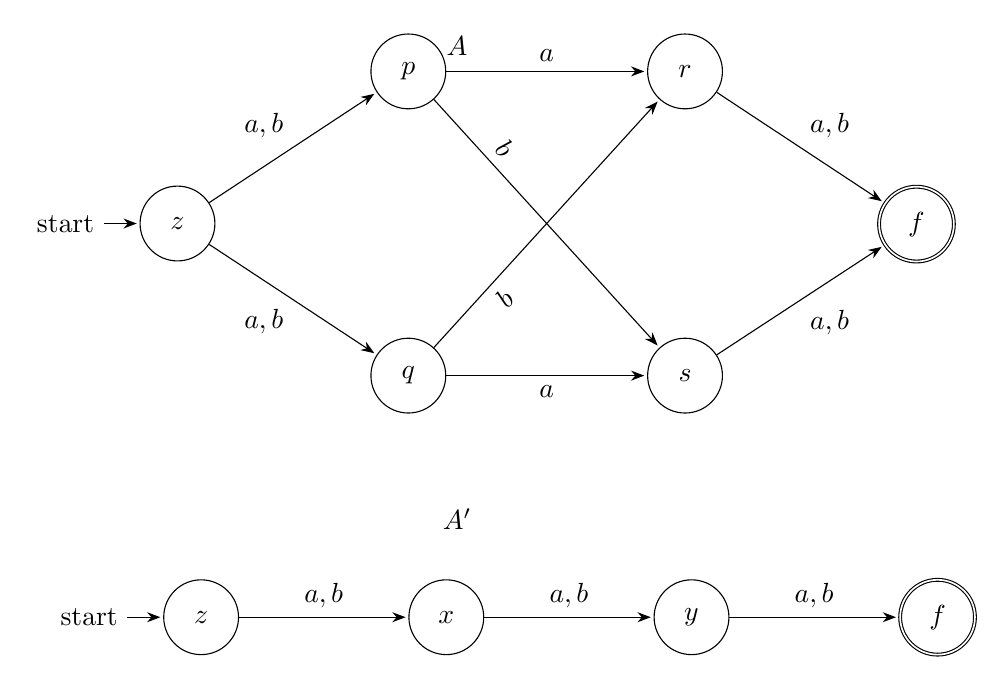
\begin{tikzpicture}[
  >=Stealth,
  shorten >=1pt,
  node distance=2.25cm and 2.6cm,
  auto,
  every state/.style={minimum size=0.95cm},
  diagram label/.style={font=\bfseries}
]
  % Original nondeterministic automaton A.  From p and q, every two-letter
  % word is accepted; from r and s, every one-letter word is accepted.
  \node[diagram label] at (3.55,2.25) {$A$};
  \node[state,initial] (z) {$z$};
  \node[state,above right=1.25cm and 2.25cm of z] (p) {$p$};
  \node[state,below right=1.25cm and 2.25cm of z] (q) {$q$};
  \node[state,right=2.55cm of p] (r) {$r$};
  \node[state,right=2.55cm of q] (s) {$s$};
  \node[state,accepting,below right=1.25cm and 2.25cm of r] (f) {$f$};

  \path[->]
    (z) edge node[above left] {$a,b$} (p)
        edge node[below left] {$a,b$} (q)
    (p) edge node[above] {$a$} (r)
        edge node[pos=.25,above,sloped] {$b$} (s)
    (q) edge node[pos=.25,below,sloped] {$b$} (r)
        edge node[below] {$a$} (s)
    (r) edge node[above right] {$a,b$} (f)
    (s) edge node[below right] {$a,b$} (f);

  % Reduced automaton A': p,q merge into x and r,s merge into y.
  \begin{scope}[xshift=0.3cm,yshift=-5cm]
    \node[diagram label] at (3.25,1.25) {$A'$};
    \node[state,initial] (zp) {$z$};
    \node[state,right=2.15cm of zp] (x) {$x$};
    \node[state,right=2.15cm of x] (y) {$y$};
    \node[state,accepting,right=2.15cm of y] (fp) {$f$};

    \path[->]
      (zp) edge node {$a,b$} (x)
      (x) edge node {$a,b$} (y)
      (y) edge node {$a,b$} (fp);
  \end{scope}
\end{tikzpicture}
\end{document}
